% !TeX program = pdflatex
% Presentacion de Deep Learning guiada por el PDF de Machine Learning.
% 19 diapositivas principales, sin anexos.
% Tiempo: 18 min de contenido + 0:30 de apertura + 1:30 de transiciones = 20 min.
% Compilar dos veces con pdfLaTeX. No requiere imagenes ni datos externos.
\PassOptionsToPackage{table}{xcolor}
\documentclass[aspectratio=169,10pt]{beamer}
\usepackage[utf8]{inputenc}
\usepackage[T1]{fontenc}
\usepackage{textcomp,lmodern}
\renewcommand{\rmdefault}{ptm}
\usefonttheme{serif}
\usepackage{amsmath,amssymb,booktabs,array,tabularx}
\usepackage{tikz,pgfplots,pgfplotstable}
\usetikzlibrary{arrows.meta,positioning,calc}
\pgfplotsset{compat=1.18}

% Colores y tipografia reconstruidos de la presentacion de referencia.
\definecolor{Azul}{rgb}{.2,.2,.7}
\definecolor{Marino}{rgb}{.1,.1,.35}
\definecolor{Tinta}{HTML}{17324D}
\definecolor{Claro}{HTML}{EDF4F7}
\definecolor{Fondo}{HTML}{F5F9FB}
\definecolor{Gris}{HTML}{596979}
\definecolor{Teal}{HTML}{087F8C}
\definecolor{Medio}{HTML}{8294A8}
\setbeamercolor{normal text}{fg=black,bg=white}
\setbeamercolor{structure}{fg=Azul}
\setbeamercolor{frametitle}{fg=white,bg=Azul}
\setbeamercolor{footline}{fg=white,bg=Marino}
\setbeamercolor{block title}{fg=Tinta,bg=Claro}
\setbeamercolor{block body}{fg=Tinta,bg=Fondo}
\setbeamerfont{block title}{family=\rmfamily,series=\bfseries,size=\normalsize}
\setbeamerfont{block body}{family=\rmfamily,size=\small}
\setbeamertemplate{blocks}[default]
\setbeamertemplate{navigation symbols}{}
\setbeamertemplate{itemize item}{\color{Azul}\scriptsize$\bullet$}
\setbeamersize{text margin left=.70cm,text margin right=.70cm}
\setbeamerfont{frametitle}{family=\sffamily,size=\fontsize{14.4}{17}\selectfont}
\setbeamertemplate{frametitle}{%
 \nointerlineskip
 \hbox to\textwidth{%
 \begin{beamercolorbox}[wd=\paperwidth,ht=18pt,dp=5.5pt,leftskip=10pt]{frametitle}
 \usebeamerfont{frametitle}\insertframetitle\strut
 \end{beamercolorbox}\hss}
 \vskip-1pt}



\setbeamerfont{footline}{family=\rmfamily,series=\bfseries,size=\fontsize{6}{7}\selectfont}
\setbeamertemplate{footline}{%
 \leavevmode\hbox{%
 \begin{beamercolorbox}[wd=.37\paperwidth,ht=7.5pt,dp=3pt,leftskip=3pt]{footline}
 \usebeamerfont{footline}By Jassan Arteta \textcopyright\ Copyright 2026.
 \end{beamercolorbox}%
 \begin{beamercolorbox}[wd=.40\paperwidth,ht=7.5pt,dp=3pt,center]{footline}
 \usebeamerfont{footline}Predicción de volatilidad con Deep Learning
 \end{beamercolorbox}%
 \begin{beamercolorbox}[wd=.13\paperwidth,ht=7.5pt,dp=3pt,center]{footline}
 \usebeamerfont{footline}2026
 \end{beamercolorbox}%
 \begin{beamercolorbox}[wd=.10\paperwidth,ht=7.5pt,dp=3pt,center]{footline}
 \usebeamerfont{footline}\insertframenumber/\inserttotalframenumber
 \end{beamercolorbox}}}
\title{Predicción de volatilidad de Bitcoin con Deep Learning}
\author{Jassan Arteta}
\date{2026}
\hypersetup{colorlinks=true,urlcolor=Teal,linkcolor=Teal,
 pdfauthor={Jassan Arteta},
 pdftitle={Predicción de volatilidad de Bitcoin con Deep Learning},
 pdfsubject={CNN-LSTM-atención; evaluación histórica con DM-HAC14 y sensibilidad HLN}}
\newcommand{\BookURL}{https://jassan-bit.github.io/DeepLearning_202630/entregable3}
\newcommand{\RawURL}{https://raw.githubusercontent.com/jassan-bit/DeepLearning_202630/main}
\newcommand{\DatosURL}{https://raw.githubusercontent.com/jassan-bit/DeepLearning_202630/8f65eac34aaf49293924ae8328c235cedbdd2866/book_e2/_static/e2_scientific_closure_20261116/data_audit/current_cohort_arrays.npz}
\newcommand{\ResultadosURL}{https://jassan-bit.github.io/DeepLearning_202630/entregable3/_static/e3_input_only_candidate_20261121/inputs/public_results.zip}
\newcommand{\ModeloURL}{\RawURL/experiments/e3_input_only_candidate_20261121/runtime/vendor/seoi_v5/model.py}
\newcommand{\tiempo}[1]{\par{\fontsize{7}{8}\selectfont\bfseries Tiempo sugerido: #1\par}\vspace{.18cm}}

\newcommand{\bajada}[1]{{\small #1\par}\smallskip}
\newcommand{\azul}[1]{\par{\color{Tinta}\bfseries #1}\par\smallskip}
\newcommand{\idea}[1]{\vfill\par\noindent\colorbox{Claro}{%
 \parbox{\dimexpr\linewidth-2\fboxsep\relax}{\small\raggedright\color{Tinta}\bfseries #1}}\par}
\newcommand{\fuente}[2]{\par\smallskip{\fontsize{6.5}{7.6}\selectfont\color{Gris}Fuente: \href{\BookURL/sections/#1.html}{#2}.\par}}
\newcommand{\fuenteURL}[2]{\par\smallskip{\fontsize{6.5}{7.6}\selectfont\color{Gris}Fuente: \href{#1}{#2}.\par}}
\newcommand{\compacta}{\setlength{\abovedisplayskip}{3pt}\setlength{\belowdisplayskip}{3pt}\setlength{\abovedisplayshortskip}{2pt}\setlength{\belowdisplayshortskip}{3pt}}
\newcolumntype{Y}{>{\raggedright\arraybackslash}X}
\newcolumntype{P}[1]{>{\raggedright\arraybackslash}p{#1}}
\renewcommand{\arraystretch}{1.10}
\newenvironment{puntos}{\begin{itemize}\setlength{\itemsep}{5pt}}{\end{itemize}}
\tikzset{caja/.style={draw=Azul!25,fill=Claro,align=center,text width=2.5cm,minimum height=.80cm,inner sep=4pt,font=\small},flecha/.style={-{Latex[length=2mm]},thick,draw=Teal}}
\pgfplotsset{every axis/.append style={
 tick label style={font=\scriptsize,color=Gris,/pgf/number format/use comma,/pgf/number format/1000 sep={}},
 label style={font=\small},title style={font=\normalsize},
 axis line style={gray!40},grid style={gray!18},
 legend style={draw=none,fill=white,font=\scriptsize},scaled ticks=false}}
\setlength{\emergencystretch}{1em}

% Serie real de las barras unicas presentes en las ventanas de ajuste.
% day: dias desde 01/01/2023; closek: miles de USDT; returnpct: 100*log(Ct/Ct-1).
% nan conserva los huecos del calendario.
\pgfplotstableread[row sep=\\]{
day closek returnpct\\
0 16.616750 nan\\
1 16.672870 0.337162\\
2 16.675180 0.013854\\
3 16.850360 1.045064\\
4 16.831850 -0.109910\\
5 16.950650 0.703326\\
6 16.943570 -0.041777\\
7 17.127830 1.081622\\
8 17.178260 0.294000\\
9 17.440660 1.515963\\
10 17.943260 2.841030\\
11 18.846620 4.911903\\
12 19.930010 5.589305\\
13 20.954920 5.014683\\
14 20.871500 -0.398887\\
15 21.185650 1.493947\\
16 21.134810 -0.240262\\
17 20.677470 -2.187674\\
18 21.071590 1.888099\\
19 22.667210 7.299370\\
20 22.783550 0.511940\\
21 22.707880 -0.332678\\
22 22.916450 0.914299\\
23 22.632890 -1.245084\\
24 23.060940 1.873612\\
25 23.009650 -0.222658\\
26 23.074160 0.279968\\
27 23.022600 -0.223703\\
28 23.742300 3.078193\\
29 22.826150 -3.935146\\
30 23.125130 1.301310\\
31 23.732660 2.593225\\
32 23.488940 -1.032249\\
33 23.431900 -0.243133\\
34 23.326840 -0.449371\\
35 22.932910 -1.703163\\
36 22.762520 -0.745767\\
37 23.240460 2.077940\\
38 22.963000 -1.201050\\
39 21.796350 -5.214170\\
40 21.625190 -0.788369\\
41 21.862550 1.091629\\
42 21.783540 -0.362049\\
43 21.773970 -0.043942\\
44 22.199840 1.936986\\
45 24.324050 9.138049\\
46 23.517720 -3.371139\\
47 24.569970 4.377079\\
48 24.631950 0.251942\\
49 24.271760 -1.473085\\
50 24.842200 2.323029\\
51 24.452160 -1.582526\\
52 24.182210 -1.110132\\
53 23.940200 -1.005818\\
54 23.185290 -3.204103\\
55 23.157070 -0.121789\\
56 23.554850 1.703161\\
57 23.492090 -0.266798\\
58 23.141570 -1.503320\\
59 23.628970 2.084293\\
60 23.465320 -0.694992\\
61 22.354340 -4.850310\\
62 22.346570 -0.034764\\
63 22.430240 0.373721\\
64 22.410000 -0.090276\\
65 22.197960 -0.950690\\
66 21.705440 -2.243747\\
67 20.362220 -6.388170\\
68 20.150690 -1.044269\\
69 20.455730 1.502451\\
70 21.997110 7.264804\\
71 24.113480 9.185994\\
72 24.670410 2.283353\\
73 24.285660 -1.571850\\
74 24.998780 2.894097\\
75 27.395130 9.153824\\
76 26.907490 -1.796057\\
77 27.972870 3.883043\\
78 27.717010 -0.918881\\
79 28.105470 1.391792\\
80 27.250970 -3.087510\\
81 nan nan\\
82 nan nan\\
83 27.462950 nan\\
84 27.968050 1.822496\\
85 27.124910 -3.061029\\
86 27.261070 0.500718\\
87 28.348600 3.911797\\
88 28.028530 -1.135473\\
89 28.465360 1.546499\\
90 28.452730 -0.044380\\
91 28.171870 -0.992015\\
92 27.800000 -1.328794\\
93 28.165470 1.306074\\
94 28.170010 0.016118\\
95 28.033820 -0.484630\\
96 27.906330 -0.455809\\
97 27.938380 0.114783\\
98 28.323760 1.369966\\
99 29.637340 4.533402\\
100 30.200420 1.882078\\
101 29.888070 -1.039643\\
102 30.373840 1.612231\\
103 30.466930 0.306012\\
104 30.295090 -0.565618\\
105 30.304650 0.031551\\
106 29.430270 -2.927743\\
107 30.380010 3.176109\\
108 28.797100 -5.351014\\
109 28.243650 -1.940603\\
110 27.262840 -3.534405\\
111 27.816850 2.011735\\
112 27.590600 -0.816682\\
113 27.510930 -0.289175\\
114 28.300790 2.830634\\
115 28.415290 0.403766\\
116 29.472770 3.653941\\
117 29.311700 -0.548003\\
118 29.230450 -0.277578\\
119 29.233210 0.009442\\
120 28.068260 -4.066599\\
121 28.669860 2.120700\\
122 29.026160 1.235110\\
123 28.838160 -0.649798\\
124 29.505610 2.288090\\
125 28.848200 -2.253282\\
126 28.430100 -1.459916\\
127 27.668790 -2.714338\\
128 27.628270 -0.146554\\
129 27.598750 -0.106904\\
130 26.968620 -2.309651\\
131 26.795010 -0.645829\\
132 26.775280 -0.073660\\
133 26.917620 0.530202\\
134 27.162140 0.904300\\
135 27.033840 -0.473468\\
136 27.405610 1.365832\\
137 26.821280 -2.155213\\
138 26.880260 0.219659\\
139 27.102430 0.823120\\
140 26.747780 -1.317191\\
141 26.849270 0.378715\\
142 27.219610 1.369904\\
143 26.329010 -3.326630\\
144 26.473790 0.548381\\
145 26.705920 0.873008\\
146 26.854270 0.553958\\
147 28.065000 4.409841\\
148 27.736400 -1.177762\\
149 27.694400 -0.151540\\
150 27.210350 -1.763281\\
151 26.817930 -1.452672\\
152 27.242590 1.571086\\
153 27.069220 -0.638427\\
154 27.115210 0.169754\\
155 25.728200 -5.250716\\
156 27.230080 5.673458\\
157 26.339340 -3.325861\\
158 26.498610 0.602864\\
159 26.477810 -0.078526\\
160 25.841210 -2.433652\\
161 25.925550 0.325846\\
162 25.905190 -0.078563\\
163 25.934250 0.112115\\
164 25.128600 -3.155785\\
165 25.598490 1.852673\\
166 26.345000 2.874514\\
167 26.516990 0.650716\\
168 26.339970 -0.669810\\
169 26.844350 1.896781\\
170 28.307990 5.308873\\
171 29.993890 5.784960\\
172 29.884920 -0.363969\\
173 30.688500 2.653399\\
174 30.527430 -0.526237\\
175 30.462660 -0.212395\\
176 30.267990 -0.641095\\
177 30.692440 1.392565\\
178 30.077410 -2.024198\\
179 30.447310 1.222326\\
180 30.472000 0.081058\\
181 30.585900 0.373089\\
182 30.617030 0.101727\\
183 31.156200 1.745687\\
184 30.766510 -1.258650\\
185 30.504810 -0.854238\\
186 29.895430 -2.017875\\
187 30.344700 1.491625\\
188 30.284630 -0.198155\\
189 30.160710 -0.410024\\
190 30.411570 0.828304\\
191 30.622100 0.689884\\
192 30.380000 -0.793747\\
193 31.454230 3.474898\\
194 30.312010 -3.698947\\
195 30.289520 -0.074223\\
196 30.231990 -0.190114\\
197 30.138000 -0.311380\\
198 29.859130 -0.929618\\
199 29.909210 0.167580\\
200 29.800000 -0.365807\\
201 29.901720 0.340761\\
202 29.794000 -0.360897\\
203 30.083750 0.967813\\
204 29.176500 -3.062157\\
205 29.228910 0.179470\\
206 29.351960 0.420104\\
207 29.222780 -0.441078\\
208 29.314140 0.312145\\
209 29.352900 0.132136\\
210 29.281090 -0.244943\\
211 29.232250 -0.166936\\
212 29.705990 1.607616\\
213 29.186010 -1.765922\\
214 29.193640 0.026139\\
215 29.113990 -0.273206\\
216 29.072130 -0.143883\\
217 29.088420 0.056017\\
218 29.211060 0.420725\\
219 29.770420 1.896788\\
220 29.581990 -0.634955\\
221 29.455750 -0.427659\\
222 29.426030 -0.100948\\
223 29.430170 0.014068\\
224 29.303840 -0.430177\\
225 29.430930 0.432760\\
226 29.200000 -0.787745\\
227 28.730510 -1.620908\\
228 26.623410 -7.616872\\
229 26.054000 -2.161960\\
230 26.100010 0.176439\\
231 26.189990 0.344158\\
232 26.126920 -0.241108\\
233 26.056000 -0.271813\\
234 26.432720 1.435457\\
235 26.180050 -0.960497\\
236 26.060010 -0.459571\\
237 26.017370 -0.163756\\
238 26.101770 0.323874\\
239 26.120000 0.069818\\
240 27.716340 5.932083\\
241 27.299990 -1.513580\\
242 25.940780 -5.107009\\
243 25.805050 -0.524604\\
244 25.869510 0.249485\\
245 25.971210 0.392356\\
246 25.826020 -0.560611\\
247 25.792100 -0.131427\\
248 25.759950 -0.124728\\
249 26.255000 1.903549\\
250 25.910500 -1.320816\\
251 25.901610 -0.034316\\
252 25.841610 -0.231915\\
253 25.162520 -2.663040\\
254 25.840100 2.657196\\
255 26.222000 1.467120\\
256 26.522730 1.140335\\
257 26.600000 0.290911\\
258 26.559670 -0.151732\\
259 26.527510 -0.121159\\
260 26.762510 0.881972\\
261 27.210260 1.659208\\
262 27.125000 -0.313830\\
263 26.568080 -2.074532\\
264 26.580140 0.045383\\
265 26.575960 -0.015727\\
266 26.248380 -1.240277\\
267 26.304810 0.214754\\
268 26.221670 -0.316564\\
269 26.372990 0.575421\\
270 27.021390 2.428839\\
271 26.906960 -0.424379\\
272 26.962560 0.206425\\
273 27.992570 3.748988\\
274 27.494510 -1.795277\\
275 27.426460 -0.247811\\
276 27.778570 1.275662\\
277 27.410390 -1.334272\\
278 27.931090 1.881827\\
279 27.956670 0.091541\\
280 27.917050 -0.141820\\
281 27.590120 -1.177988\\
282 27.390120 -0.727537\\
283 26.875520 -1.896653\\
284 26.759630 -0.432143\\
285 26.862000 0.381824\\
286 26.852480 -0.035447\\
287 27.154150 1.117171\\
288 28.500780 4.840157\\
289 28.395910 -0.368633\\
290 28.320000 -0.267685\\
291 28.713710 1.380644\\
292 29.669040 3.272937\\
293 29.909800 0.808211\\
294 29.992460 0.275983\\
295 33.069990 9.768021\\
296 33.922730 2.545907\\
297 34.496050 1.675953\\
298 34.151660 -1.003363\\
299 33.892020 -0.763161\\
300 34.081000 0.556046\\
301 34.525890 1.296943\\
302 34.474730 -0.148289\\
303 34.639770 0.477585\\
304 35.421430 2.231456\\
305 34.941590 -1.363919\\
306 34.716780 -0.645467\\
307 35.062070 0.989678\\
308 35.011880 -0.143249\\
309 35.046090 0.097662\\
310 35.399120 1.002291\\
311 35.624720 0.635282\\
312 36.701090 2.976668\\
313 37.301630 1.623057\\
314 37.130000 -0.461176\\
315 37.064130 -0.177561\\
316 36.462930 -1.635353\\
317 35.551190 -2.532250\\
318 37.858200 6.287397\\
319 36.163510 -4.579700\\
320 36.613920 1.237790\\
321 36.568100 -0.125222\\
322 37.359860 2.142059\\
323 37.448780 0.237727\\
324 35.741650 -4.665746\\
325 37.408340 4.557700\\
326 37.294280 -0.305371\\
327 37.713570 1.118001\\
328 37.780670 0.177762\\
329 37.447430 -0.885951\\
330 37.242700 -0.548213\\
331 37.818870 1.535223\\
332 37.854640 0.094538\\
333 37.723960 -0.345813\\
334 38.682520 2.509238\\
335 39.450350 1.965510\\
336 39.972260 1.314279\\
337 41.991100 4.927198\\
338 44.073320 4.839692\\
339 43.762690 -0.707298\\
340 43.273140 -1.124951\\
341 44.170990 2.053612\\
342 43.713600 -1.040897\\
343 43.789510 0.173502\\
344 41.253400 -5.966076\\
345 41.492390 0.577650\\
346 42.869030 3.263962\\
347 43.022260 0.356800\\
348 41.940300 -2.547048\\
349 42.278030 0.802039\\
350 41.374650 -2.159919\\
351 42.657800 3.054177\\
352 42.275990 -0.899083\\
353 43.668930 3.241755\\
354 43.861800 0.440692\\
355 43.969040 0.244197\\
356 43.702160 -0.608822\\
357 42.991500 -1.639511\\
358 43.576130 1.350710\\
359 42.508930 -2.479535\\
360 43.428850 2.140980\\
361 42.563760 -2.012078\\
362 42.066950 -1.174079\\
363 42.140280 0.174166\\
364 42.283580 0.339478\\
365 44.179550 4.386318\\
366 44.946910 1.722000\\
367 42.845230 -4.788770\\
368 44.151100 3.002352\\
369 44.145110 -0.013568\\
370 43.968320 -0.401279\\
371 43.929020 -0.089423\\
372 46.951040 6.653021\\
373 46.110000 -1.807551\\
374 46.653990 1.172861\\
375 46.339160 -0.677106\\
376 42.782730 -7.985288\\
377 42.847990 0.152422\\
378 41.732350 -2.638213\\
379 42.511100 1.848861\\
380 43.137950 1.463790\\
381 42.776100 -0.842358\\
382 41.327500 -3.445140\\
383 41.659030 0.799001\\
384 41.696040 0.088801\\
385 41.580330 -0.277894\\
386 39.568020 -4.960600\\
387 39.897600 0.829496\\
388 40.084880 0.468303\\
389 39.961090 -0.309298\\
390 41.823510 4.555239\\
391 42.120630 0.707902\\
392 42.031060 -0.212878\\
393 43.302700 2.980612\\
394 42.941100 -0.838558\\
395 42.580000 -0.844475\\
396 43.082940 1.174244\\
397 43.200000 0.271340\\
398 43.011090 -0.438251\\
399 42.582880 -1.000569\\
400 42.708700 0.295035\\
401 43.098950 0.909599\\
402 44.349600 2.860505\\
403 45.288650 2.095276\\
404 47.132770 3.991206\\
405 47.751090 1.303338\\
406 48.299990 1.142946\\
407 49.917270 3.293568\\
408 49.699590 -0.437035\\
409 51.795170 4.130022\\
410 51.880000 0.163646\\
411 52.124110 0.469425\\
412 51.642640 -0.927992\\
413 52.137670 0.954003\\
414 51.774730 -0.698553\\
415 52.258820 0.930649\\
416 51.849390 -0.786551\\
417 51.288420 -1.087817\\
418 50.744150 -1.066866\\
419 51.568220 1.610925\\
420 51.728850 0.311006\\
421 54.476470 5.175321\\
422 57.037340 4.593728\\
423 62.432100 9.037343\\
424 61.130980 -2.106079\\
425 62.387900 2.035257\\
426 61.987280 -0.644214\\
427 63.113970 1.801294\\
428 68.245710 7.817244\\
429 63.724010 -6.855316\\
430 66.074040 3.621452\\
431 66.823170 1.127395\\
432 68.124190 1.928249\\
433 68.313270 0.277167\\
434 68.955880 0.936284\\
435 72.078100 4.428337\\
436 71.452010 -0.872422\\
437 73.072410 2.242483\\
438 71.388940 -2.330791\\
439 69.499850 -2.681836\\
440 65.300630 -6.232291\\
441 68.393480 4.627581\\
442 67.609990 -1.152175\\
443 61.937400 -8.763156\\
444 67.840510 9.103531\\
445 65.501270 -3.508998\\
446 63.796640 -2.636901\\
447 63.990010 0.302645\\
448 67.209990 4.909492\\
449 69.880010 3.895773\\
450 69.988000 0.154417\\
451 69.469990 -0.742894\\
452 70.780600 1.869009\\
453 69.850540 -1.322714\\
454 69.582180 -0.384932\\
455 71.280010 2.410742\\
456 69.649800 -2.313609\\
457 65.463990 -6.197961\\
458 65.963280 0.759800\\
459 68.487790 3.755726\\
460 67.820620 -0.978920\\
461 68.896000 1.573184\\
462 69.360390 0.671783\\
463 71.620000 3.205841\\
464 69.146000 -3.515415\\
465 70.631080 2.125006\\
466 70.006230 -0.888604\\
467 67.116520 -4.215402\\
468 63.924510 -4.872736\\
469 65.661840 2.681508\\
470 63.419990 -3.473882\\
471 63.793390 0.587047\\
472 61.277370 -4.023897\\
473 63.470080 3.515801\\
474 63.818010 0.546683\\
475 64.940590 1.743741\\
476 64.941150 0.000862\\
477 66.819320 2.851079\\
478 66.414000 -0.608438\\
479 64.289590 -3.251016\\
480 64.498340 0.324177\\
481 63.770010 -1.135647\\
482 63.461980 -0.484203\\
483 63.118620 -0.542517\\
484 63.866000 1.177133\\
485 60.672000 -5.130483\\
486 58.364970 -3.876643\\
487 59.060610 1.184832\\
488 62.882010 6.269591\\
489 63.892040 1.593467\\
490 64.012000 0.187578\\
491 63.165190 -1.331721\\
492 62.312080 -1.359805\\
493 61.193030 -1.812201\\
494 63.074010 3.027550\\
495 60.799990 -3.671917\\
496 60.825990 0.042754\\
497 61.483990 1.075965\\
498 62.940080 2.340635\\
499 61.577490 -2.188678\\
500 66.206500 7.248226\\
501 65.235210 -1.477929\\
502 67.024000 2.705141\\
503 66.915200 -0.162462\\
504 66.274010 -0.962833\\
505 71.446620 7.515278\\
506 70.148340 -1.833845\\
507 69.166620 -1.409377\\
508 67.969650 -1.745709\\
509 68.549990 0.850198\\
510 69.290570 1.074556\\
511 68.507670 -1.136311\\
512 69.436430 1.346595\\
513 68.398390 -1.506237\\
514 67.652420 -1.096616\\
515 68.352170 1.029018\\
516 67.540010 -1.195315\\
517 67.766850 0.335297\\
518 67.765630 -0.001800\\
519 68.809900 1.529250\\
520 70.537840 2.480167\\
521 71.108000 0.805054\\
522 70.799060 -0.435412\\
523 69.355600 -2.059883\\
524 69.310460 -0.065106\\
525 69.648140 0.486016\\
526 69.540000 -0.155387\\
527 67.314240 -3.253032\\
528 68.263990 1.401059\\
529 66.773010 -2.208344\\
530 66.043990 -1.097792\\
531 66.228250 0.278607\\
532 66.676870 0.675101\\
533 66.504330 -0.259106\\
534 65.175320 -2.018619\\
535 64.974370 -0.308799\\
536 64.869990 -0.160777\\
537 64.143560 -1.126142\\
538 64.262010 0.184494\\
539 63.210010 -1.650596\\
540 60.293300 -4.724169\\
541 61.806010 2.477962\\
542 60.864990 -1.534248\\
543 61.706470 1.373066\\
544 60.427840 -2.093886\\
545 60.986680 0.920555\\
}\SerieAjuste

\newcommand{\HistURL}{\BookURL/_static/e3_estadistica_posterior_20261117}

% Análisis complementario del 25/11/2026: misma cohorte histórica de 608 fechas.
\newcommand{\DMURL}{\BookURL/sections/08_verificacion_estadistica.html\#e3-dm-hln-20261125}

\begin{document}
\raggedright
\begin{frame}[t]
% Apertura: 0:30. Contenido: 18:00. Transiciones: 1:30. Total: 20:00.
\vspace{.95cm}
\begin{beamercolorbox}[wd=\textwidth,sep=6pt,center]{frametitle}
{\sffamily\fontsize{17.2}{21.2}\selectfont
PREDICCIÓN DE VOLATILIDAD DE BITCOIN\\CON DEEP LEARNING}
\end{beamercolorbox}
\vspace{.22cm}
{\color{Gris}CNN--LSTM con atención y salida estructurada\par}
\vspace{.42cm}
{\fontsize{13}{16}\selectfont Jassan Arteta\par}
\smallskip
Universidad del Norte\enspace |\enspace Maestría en Matemáticas
\vspace{.35cm}
\idea{¿Qué aporta aprender la magnitud futura y aprovechar la parte de la volatilidad que ya se conoce?}
\vspace{.40cm}
\end{frame}

\begin{frame}[t]{Problema y objetivos}
\tiempo{0:30}\compacta
\begin{puntos}
\item \textbf{Objetivo:} anticipar la volatilidad de Bitcoin al cierre del siguiente día.
\item Usar siete días de apertura, máximo, mínimo, cierre y volumen (OHLCV).
\item Comparar una red con salida estructurada frente a variantes y controles simples.
\end{puntos}
\medskip
\begin{center}
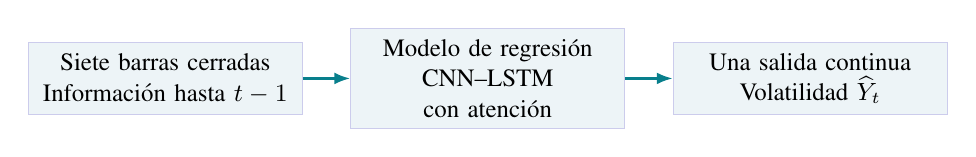
\begin{tikzpicture}
\node[caja,text width=3.2cm] (x) {Siete barras cerradas\\Información hasta $t-1$};
\node[caja,text width=3.2cm,right=6mm of x] (m) {Modelo de regresión\\CNN--LSTM con atención};
\node[caja,text width=3.2cm,right=6mm of m] (y) {Una salida continua\\Volatilidad $\widehat Y_t$};
\draw[flecha] (x)--(m);\draw[flecha] (m)--(y);
\end{tikzpicture}
\end{center}
{\footnotesize CNN: red neuronal convolucional. LSTM: memoria de corto y largo plazo.}
\idea{El aprendizaje profundo permite representar relaciones temporales no lineales. Su utilidad predictiva se evalúa con los mismos objetivos y fechas.}
\fuente{01_introduccion}{Problema y contrato de predicción del Entregable 3}
\end{frame}

\begin{frame}[t]{Datos y alcance del estudio}
\tiempo{0:30}\compacta
\begin{columns}[T,onlytextwidth]
\column{.48\textwidth}
\begin{block}{Fuente y calidad}
\begin{puntos}
\item Binance Spot: BTC frente a USDT. Barras diarias en tiempo universal coordinado (UTC).
\item Auditoría 2023--2024: 731 fechas y 730 barras completas.
\item La barra incompleta del 24/03/2023 afecta ocho objetivos. Se conservan los huecos.
\end{puntos}
\end{block}
\column{.48\textwidth}
\begin{block}{Candidata actual}
\texttt{input-only-overlap-mse-1}
\medskip\par
532 objetivos de ajuste, 54 de selección y 55 de evaluación de desarrollo.
\medskip\par
Dos purgas temporales de siete días. Las 55 fechas ya estaban expuestas durante el desarrollo.
\end{block}
\end{columns}
\idea{La arquitectura presentada es input-only: sus 55 fechas son de desarrollo. El bloque estadístico histórico usa otra versión y otras 608 fechas.}
\fuente{06_modelo_original}{Candidata actual, 6.20--6.21; calidad de datos en capítulo 4}
\end{frame}

\begin{frame}[t]{EDA: precios y retornos del ajuste}
\tiempo{0:30}\compacta
\bajada{Análisis exploratorio de datos (EDA). Barras únicas presentes en las 532 ventanas de ajuste, con huecos conservados.}
\begin{columns}[T,onlytextwidth]
\column{.49\textwidth}
\begin{tikzpicture}
\begin{axis}[width=\dimexpr\linewidth-4pt\relax,height=3.65cm,title={Cierre diario conocido},
xmin=0,xmax=545,xtick={0,181,365,545},xticklabels={ene.23,jul.23,ene.24,jun.24},
ylabel={Miles de USDT},xlabel={Fecha UTC},grid=major,unbounded coords=jump]
\addplot[Tinta,thin,no marks] table[x=day,y=closek] {\SerieAjuste};
\end{axis}
\end{tikzpicture}
\column{.49\textwidth}
\begin{tikzpicture}
\begin{axis}[width=\dimexpr\linewidth-4pt\relax,height=3.65cm,title={Retorno logarítmico diario},
xmin=0,xmax=545,xtick={0,181,365,545},xticklabels={ene.23,jul.23,ene.24,jun.24},
ylabel={Retorno (\%)},xlabel={Fecha UTC},grid=major,unbounded coords=jump]
\addplot[Teal,thin,no marks] table[x=day,y=returnpct] {\SerieAjuste};
\end{axis}
\end{tikzpicture}
\end{columns}
{\small 544 cierres y 542 retornos entre días consecutivos. $r_t=\log(C_t/C_{t-1})$; el gráfico muestra $100r_t$.}
\idea{El precio cambia de nivel durante el periodo. Los retornos permiten comparar la magnitud de los movimientos y muestran episodios de amplitud diferente.}
\fuenteURL{\DatosURL}{Cálculo descriptivo sobre las barras originales de las ventanas de ajuste}
\end{frame}

\begin{frame}[t]{EDA: distribución de la volatilidad objetivo}
\tiempo{0:30}\compacta
\bajada{532 objetivos de ajuste, del 08/01/2023 al 30/06/2024. Volatilidad poblacional sin anualizar.}
\begin{columns}[T,onlytextwidth]
\column{.66\textwidth}
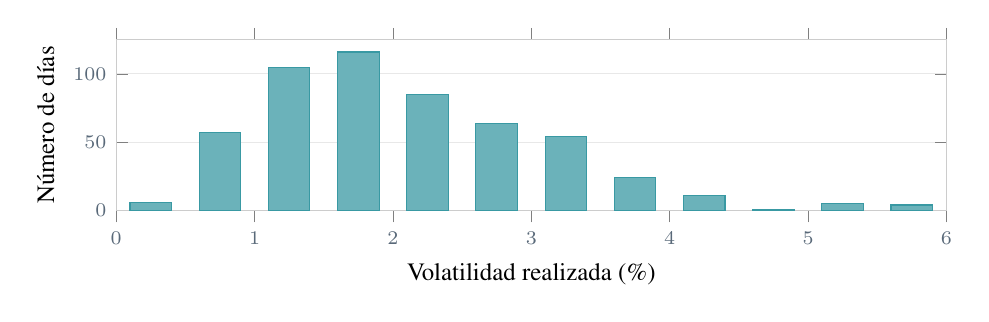
\begin{tikzpicture}
\begin{axis}[ybar,width=\linewidth,height=3.75cm,xmin=0,xmax=6,ymin=0,ymax=125,
xtick={0,1,2,3,4,5,6},xlabel={Volatilidad realizada (\%)},ylabel={Número de días},
bar width=15pt,ymajorgrids]
\addplot[fill=Teal!60,draw=Teal!80] coordinates {(0.25,6) (0.75,57) (1.25,105) (1.75,116) (2.25,85) (2.75,64) (3.25,54) (3.75,24) (4.25,11) (4.75,1) (5.25,5) (5.75,4)};
\end{axis}
\end{tikzpicture}
\column{.30\textwidth}
\begin{tabular}{lr}
\toprule Medida & Valor\\\midrule
Mediana & 1,94\%\\
Percentil 95 & 3,85\%\\
Máximo & 5,73\%\\\bottomrule
\end{tabular}
\medskip\par
Diez alertas por encima de $Q_3+1{,}5\,\mathrm{IQR}$, donde IQR es el rango intercuartílico.
\end{columns}
\idea{La distribución presenta cola derecha y pocos episodios extremos. Estas observaciones se conservan porque forman parte del problema de predicción.}
\fuenteURL{\RawURL/data/e3_dashboard_v1/observations.csv}{Cálculo sobre los 532 objetivos de ajuste publicados}
\end{frame}

\begin{frame}[t]{EDA temporal: retornos y retornos al cuadrado}
\tiempo{0:30}\compacta
\bajada{Función de autocorrelación (ACF) con rezagos en días de calendario. Los huecos permanecen en su fecha.}
\begin{columns}[T,onlytextwidth]
\column{.49\textwidth}
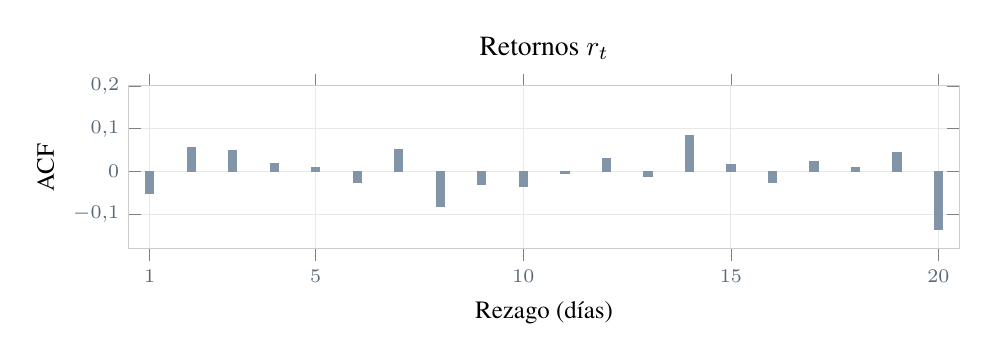
\begin{tikzpicture}
\begin{axis}[ybar,width=\linewidth,height=3.65cm,title={Retornos $r_t$},xmin=.5,xmax=20.5,
ymin=-.18,ymax=.20,xtick={1,5,10,15,20},ytick={-.1,0,.1,.2},xlabel={Rezago (días)},ylabel={ACF},bar width=3pt,grid=major]
\addplot[fill=Medio,draw=Medio] coordinates {(1,-0.052001) (2,0.057280) (3,0.048447) (4,0.019428) (5,0.008724) (6,-0.024503) (7,0.051892) (8,-0.081539) (9,-0.029727) (10,-0.035553) (11,-0.004876) (12,0.029848) (13,-0.010447) (14,0.085307) (15,0.015647) (16,-0.024225) (17,0.023608) (18,0.010308) (19,0.043723) (20,-0.135157)};
\end{axis}
\end{tikzpicture}
\column{.49\textwidth}
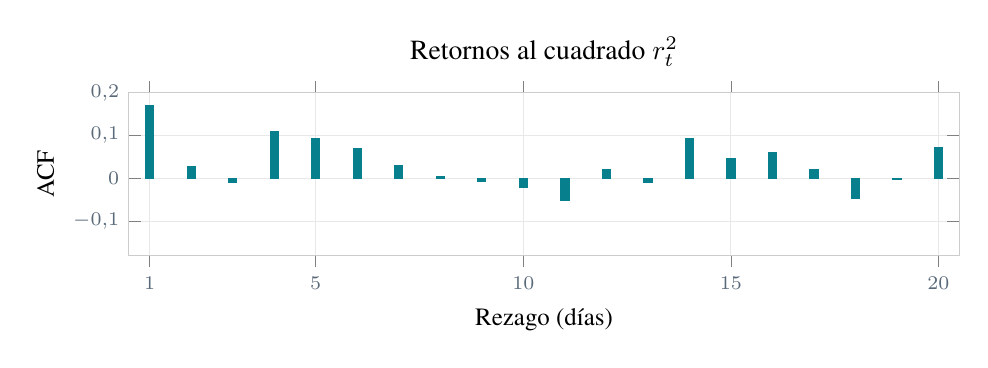
\begin{tikzpicture}
\begin{axis}[ybar,width=\linewidth,height=3.65cm,title={Retornos al cuadrado $r_t^2$},xmin=.5,xmax=20.5,
ymin=-.18,ymax=.20,xtick={1,5,10,15,20},ytick={-.1,0,.1,.2},xlabel={Rezago (días)},ylabel={ACF},bar width=3pt,grid=major]
\addplot[fill=Teal,draw=Teal] coordinates {(1,0.170906) (2,0.026767) (3,-0.010036) (4,0.108465) (5,0.092255) (6,0.070080) (7,0.030803) (8,0.004971) (9,-0.006569) (10,-0.021401) (11,-0.050811) (12,0.020388) (13,-0.010543) (14,0.092025) (15,0.045132) (16,0.059797) (17,0.020109) (18,-0.046170) (19,-0.001792) (20,0.073000)};
\end{axis}
\end{tikzpicture}
\end{columns}
{\small Primer rezago: $-0{,}0520$ en retornos y $0{,}1709$ en retornos al cuadrado. Cálculo descriptivo sin bandas inferenciales.}
\idea{Los retornos al cuadrado muestran mayor autocorrelación en el primer rezago. Esto motiva evaluar información temporal, sin demostrar estacionariedad ni ventaja predictiva.}
\fuenteURL{\DatosURL}{Pares válidos separados por días reales}
\end{frame}

\begin{frame}[t]{Ventana de entrada, objetivo y horizonte}
\tiempo{1:00}\compacta
\begin{columns}[T,onlytextwidth]
\column{.48\textwidth}
\begin{block}{Entrada y frecuencia}
Siete barras diarias OHLCV:
\[
X_t\in\mathbb R^{7\times5}.
\]
La información llega hasta el cierre de $t-1$. La salida corresponde al día $t$.
\end{block}
\begin{block}{Horizonte}
\textbf{Un día.} Una predicción por fecha de origen, con la misma definición de volatilidad.
\end{block}
\column{.48\textwidth}
\begin{block}{Ventana del objetivo}
Siete retornos logarítmicos:
\[
Y_t=\sqrt{\frac17\sum_{i=t-6}^{t}(r_i-\bar r_t)^2}.
\]
$r_i=\log(C_i/C_{i-1})$ y $\bar r_t$ es su media.
\medskip\par
Siete retornos requieren ocho cierres. Al pronosticar, seis retornos ya son conocidos.
\end{block}
\end{columns}
\idea{La ventana mide volatilidad sobre siete retornos y el horizonte indica cuánto se adelanta el pronóstico. El solapamiento permite usar explícitamente la parte conocida del objetivo.}
\fuente{06_modelo_original}{Contrato de entrada y descomposición de la etiqueta}
\end{frame}

\begin{frame}[t]{Preprocesamiento y prevención de fuga de información}
\tiempo{1:00}\compacta
\begin{columns}[T,onlytextwidth]
\column{.49\textwidth}
\azul{Precios relativos y escala local}
\[
F_{j,P}=\frac{\log P_j-\log C_{\rm last}}{s_t},
\]
\[
s_t=\max\!\left(\sqrt{\frac16\sum_{i=1}^{6}r_i^2},10^{-6}r_{\rm fit}\right).
\]
{\small $P$: apertura, máximo, mínimo o cierre. $r_{\rm fit}$: escala de referencia del ajuste.}
\column{.47\textwidth}
\azul{Volumen y estandarización}
\[
F_{j,V}=\log(1+V_j),
\]
\[
x_{j,d}=\frac{F_{j,d}-\mu_{d,\rm fit}}{\sigma_{d,\rm fit}}.
\]
\begin{puntos}
\item Medias y desviaciones calculadas sólo en ajuste y luego congeladas.
\item La parte conocida del objetivo usa los retornos originales.
\end{puntos}
\end{columns}
\idea{La normalización compara formas de precio con distintas escalas. Cada ventana utiliza únicamente barras disponibles al emitir el pronóstico.}
\fuenteURL{\RawURL/experiments/e3_input_only_candidate_20261121/runtime/vendor/seoi_v5/data.py}{Transformaciones efectivas de input-only}
\end{frame}

\begin{frame}[t]{Qué aporta la salida estructurada}
\tiempo{1:15}\compacta
\begin{columns}[T,onlytextwidth]
\column{.48\textwidth}
\begin{block}{Información ya conocida}
Seis retornos determinan
\[
m_6=\frac16\sum_{i=1}^{6}r_i,\qquad
A=\frac17\sum_{i=1}^{6}(r_i-m_6)^2.
\]
$\sqrt A$ es un mínimo observable para la volatilidad futura.
\end{block}
\column{.48\textwidth}
\begin{block}{Magnitud que falta por observar}
\[
U=|r_7-m_6|.
\]
La red produce tres magnitudes $u_k>0$ y pesos $p_k>0$ que suman uno.
\medskip\par
Cada magnitud pasa por la transformación del objetivo antes del promedio.
\end{block}
\end{columns}
\[
\boxed{\widehat Y=\sum_{k=1}^{3}p_k\sqrt{A+\frac6{49}u_k^2}}
\]
\idea{El mecanismo combina la parte observada del objetivo con una representación de la magnitud futura. La MSE supervisa el pronóstico puntual y no identifica toda la distribución latente.}
\fuente{06_modelo_original}{Expediente del mecanismo, secciones 6.20--6.21}
\end{frame}

\begin{frame}[t]{CNN--LSTM con atención: arquitectura y función}
\tiempo{1:15}\compacta
\begin{center}
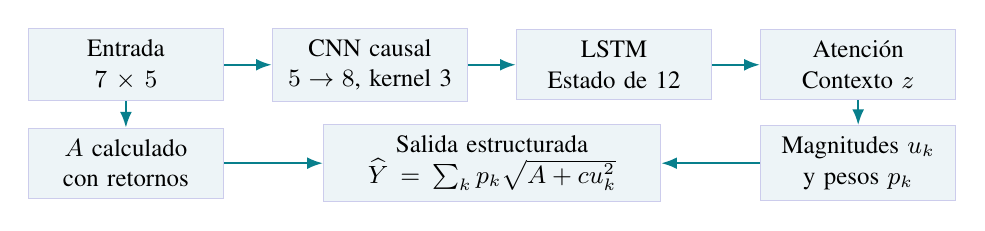
\begin{tikzpicture}
\node[caja,text width=2.2cm] (x) at(0,0) {Entrada\\$7\times5$};
\node[caja,text width=2.2cm] (c) at(3.1,0) {CNN causal\\$5\to8$, kernel 3};
\node[caja,text width=2.2cm] (l) at(6.2,0) {LSTM\\Estado de 12};
\node[caja,text width=2.2cm] (a) at(9.3,0) {Atención\\Contexto $z$};
\node[caja,text width=2.2cm] (k) at(0,-1.25) {$A$ calculado\\con retornos};
\node[caja,text width=4cm] (y) at(4.65,-1.25) {Salida estructurada\\$\widehat Y=\sum_kp_k\sqrt{A+cu_k^2}$};
\node[caja,text width=2.2cm] (u) at(9.3,-1.25) {Magnitudes $u_k$\\y pesos $p_k$};
\draw[flecha](x)--(c);\draw[flecha](c)--(l);\draw[flecha](l)--(a);
\draw[flecha](a)--(u);\draw[flecha](u)--(y);\draw[flecha](k)--(y);\draw[flecha](x)--(k);
\end{tikzpicture}
\end{center}
{\small CNN: red convolucional, extrae patrones locales. LSTM: memoria de corto y largo plazo, conserva información de la secuencia. La atención pondera los siete estados.}
\smallskip
\textbf{1.262 parámetros:} 128 CNN, 1.056 LSTM, 13 atención y 65 salida.
\idea{La red aprende una representación temporal y la rama analítica conserva la información conocida.}
\fuente{06_modelo_original}{Arquitectura de la candidata y correspondencia con el código}
\end{frame}

\begin{frame}[t]{Demostración del mínimo observable}
\tiempo{1:30}\compacta
La media de los siete retornos es $m_7=(6m_6+r_7)/7$. Por tanto,
\[
m_7-m_6=\frac{r_7-m_6}{7},\qquad
r_7-m_7=\frac67(r_7-m_6).
\]
Como $\sum_{i=1}^{6}(r_i-m_6)=0$, el término cruzado desaparece:
\[
\sum_{i=1}^{7}(r_i-m_7)^2
=\sum_{i=1}^{6}(r_i-m_6)^2+\frac67(r_7-m_6)^2.
\]
Al dividir entre siete: $Y^2=A+\frac6{49}U^2$. En la salida del modelo,
\[
\widehat Y=\sum_kp_k\sqrt{A+\frac6{49}u_k^2}
\ge\sum_kp_k\sqrt A=\sqrt A.
\]
\idea{La identidad usa varianza poblacional y pesos no negativos que suman uno. El mínimo está garantizado algebraicamente; la reducción del error debe comprobarse con datos.}
\fuente{06_modelo_original}{Demostración formal de la candidata actual}
\end{frame}

\begin{frame}[t]{Pérdida, retropropagación y entrenamiento}
\tiempo{1:15}\compacta
\begin{columns}[T,onlytextwidth]
\column{.49\textwidth}
\azul{Error cuadrático normalizado}
\[
L=\frac1n\sum_i\left(\frac{\widehat Y_i-Y_i}{s_Y}\right)^2,
\qquad s_Y=\overline Y_{\rm ajuste}.
\]
\[
\nabla_\theta L_i=
\frac{2(\widehat Y_i-Y_i)}{s_Y^2}\nabla_\theta\widehat Y_i.
\]
{\small La regla de la cadena recorre la salida, la atención, los siete pasos de la LSTM y la CNN.}
\column{.47\textwidth}
\azul{Configuración efectiva}
{\small
\begin{tabularx}{\linewidth}{Y l}
\toprule Parámetro & Valor\\\midrule
Optimizador & AdamW\\
Tasa de aprendizaje & 0,003\\
Lote / épocas máximas & 32 / 40\\
Paciencia & 8 épocas\\
Norma máxima del gradiente & 1\\
Dropout / decaimiento & 0 / 0\\\bottomrule
\end{tabularx}\par}
\end{columns}
\idea{La parada temprana conserva el modelo con menor error de selección. La arquitectura pequeña limita capacidad y el recorte de gradientes controla estabilidad numérica.}
\fuenteURL{\ResultadosURL}{Protocolo de entrenamiento}
\end{frame}

\begin{frame}[t]{Predicción registrada y explicación local}
\tiempo{1:15}\compacta
\bajada{Input-only, semilla 20261127. Predicciones originales sobre las 55 fechas de desarrollo.}
\begin{columns}[T,onlytextwidth]
\column{.65\textwidth}
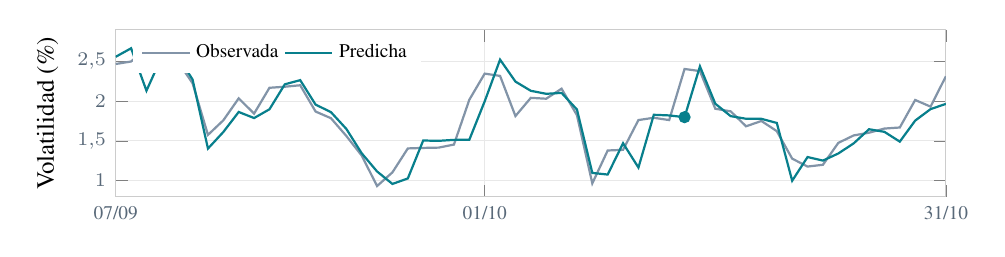
\begin{tikzpicture}
\begin{axis}[width=\linewidth,height=3.7cm,xmin=1,xmax=55,ymin=.8,ymax=2.9,
xtick={1,25,55},xticklabels={07/09,01/10,31/10},ylabel={Volatilidad (\%)},grid=major,
legend style={at={(.02,.98)},anchor=north west,legend columns=2}]
\addplot[Medio,thick,no marks] coordinates {(1,2.46839) (2,2.49964) (3,2.66619) (4,2.52755) (5,2.51070) (6,2.22569) (7,1.57550) (8,1.75946) (9,2.03594) (10,1.84373) (11,2.16878) (12,2.18211) (13,2.20080) (14,1.86983) (15,1.78578) (16,1.56234) (17,1.31563) (18,0.93182) (19,1.10454) (20,1.40544) (21,1.41178) (22,1.41561) (23,1.45413) (24,2.01821) (25,2.34722) (26,2.31839) (27,1.81294) (28,2.04222) (29,2.03117) (30,2.15738) (31,1.82362) (32,0.96544) (33,1.37930) (34,1.38767) (35,1.76264) (36,1.79143) (37,1.76228) (38,2.40578) (39,2.37913) (40,1.90504) (41,1.87241) (42,1.68391) (43,1.75092) (44,1.62257) (45,1.27666) (46,1.17717) (47,1.19949) (48,1.47506) (49,1.56903) (50,1.60345) (51,1.65555) (52,1.66901) (53,2.01529) (54,1.93163) (55,2.31422)};\addlegendentry{Observada}
\addplot[Teal,thick,no marks] coordinates {(1,2.55905) (2,2.66608) (3,2.13219) (4,2.56107) (5,2.57928) (6,2.27264) (7,1.40345) (8,1.61217) (9,1.86442) (10,1.78774) (11,1.89830) (12,2.21265) (13,2.26498) (14,1.95724) (15,1.86207) (16,1.65148) (17,1.34437) (18,1.11521) (19,0.95823) (20,1.02750) (21,1.50511) (22,1.50096) (23,1.51319) (24,1.51482) (25,1.99794) (26,2.52336) (27,2.24679) (28,2.13087) (29,2.09307) (30,2.10449) (31,1.89543) (32,1.09697) (33,1.07649) (34,1.47078) (35,1.16450) (36,1.82888) (37,1.82085) (38,1.79873) (39,2.43833) (40,1.96824) (41,1.81181) (42,1.77884) (43,1.77803) (44,1.72613) (45,0.99854) (46,1.29705) (47,1.25227) (48,1.34175) (49,1.46904) (50,1.64695) (51,1.61408) (52,1.49090) (53,1.75559) (54,1.90038) (55,1.96609)};\addlegendentry{Predicha}
\addplot[Teal,only marks,mark=*,forget plot] coordinates {(38,1.79873)};
\end{axis}
\end{tikzpicture}
\column{.31\textwidth}
\azul{14/10/2024}
\begin{tabularx}{\linewidth}{Y r}
Mínimo conocido & 1,718\%\\
Pronóstico & 1,799\%\\
Observado & 2,406\%\\
\end{tabularx}
\medskip\par
El pronóstico añade \textbf{0,081 puntos porcentuales} sobre $\sqrt A$.
\medskip\par
Error: $-0{,}607$ puntos porcentuales.
\end{columns}
\idea{La salida respeta el mínimo conocido, pero subestima el movimiento adicional de esta fecha. La descomposición explica el valor registrado sin atribuir causalidad a las entradas.}
\fuenteURL{\ResultadosURL}{predictions.csv; mínimo reconstruido de los seis retornos conocidos}
\end{frame}

\begin{frame}[t]{RMSE y Diebold--Mariano: qué compara cada prueba}
% Tiempo sugerido: 1:30.
\compacta
\bajada{CNN-LSTM-atención histórico, con salida $\sqrt A$ más un exceso aprendido. 17 sistemas y 608 fechas: 01/01/2025--31/08/2026.}
\begin{columns}[T,onlytextwidth]
\column{.48\textwidth}
\azul{Contraste previo: RMSE medio}
{\small\compacta
RMSE: raíz del error cuadrático medio. $M_m$ promedia las RMSE individuales por semilla.
\[
\Delta_j=M_j-M_{\rm CNN},\qquad H_0:\Delta_j\le\delta.
\]
$\delta=0{,}0002577284$ en unidades de RMSE.
\smallskip\par
Bootstrap por bloques de 14 días, influencia de RMSE con HAC14 y $t$ pareada entre semillas.
\smallskip\par
\textbf{Holm48: 48/48 rechazos.}\par
Rango de $p$ ajustados: $[1{,}20\times10^{-20};\,0{,}0019]$.
}
\column{.48\textwidth}
\azul{Diebold--Mariano (DM): MSE diario}
{\small\compacta
\[
\begin{aligned}
\ell_{m,t}&=\frac1{R_m}\sum_s(y_t-\widehat y_{m,s,t})^2,\\
d_t&=\ell_{{\rm CNN},t}-\ell_{j,t}.
\end{aligned}
\]
MSE: error cuadrático medio.
\[
DM=\frac{\bar d}{\sqrt{\widehat\Omega_{14}/608}},\qquad H_0:\mathbb E[d_t]=0.
\]
$h=1$. Prueba bilateral, normal asintótica.
}
\end{columns}
\smallskip
{\fontsize{8.1}{9.2}\selectfont $R_m=10$ para redes y $R_m=1$ para clásicos. $\widehat\Omega_{14}$ es la varianza de largo plazo Bartlett-HAC, que contempla heterocedasticidad y autocorrelación.\par}
\idea{El contraste previo busca una ganancia de RMSE mayor que $\delta$. DM compara pérdidas cuadráticas contra igualdad; el margen de RMSE no se traslada a MSE.}
\fuenteURL{\DMURL}{Protocolo complementario del 25/11/2026 y protocolo histórico de 48 contrastes. Ambos análisis son retrospectivos}
\end{frame}

\begin{frame}[t]{Diebold--Mariano: CNN-LSTM-atención frente a 16 rivales}
% Tiempo sugerido: 1:00. Se prioriza espacio para la tabla completa.
\compacta
\bajada{608 fechas, $h=1$. Un $DM<0$ indica menor MSE para CNN-LSTM-atención.}
{\fontsize{7.6}{8.6}\selectfont\setlength{\tabcolsep}{4pt}\renewcommand{\arraystretch}{0.88}
\begin{tabularx}{\linewidth}{@{}Yrrrr@{}}
\toprule
\textbf{Rival} & \textbf{$DM_{\rm HAC14}$} & \textbf{$p$ bruto} & \textbf{$p$ Holm16} & \textbf{$p$ Holm64}\\\midrule
\rowcolor{Fondo}LSTM-autoencoder con predictor & $-5{,}158$ & $2{,}497\times10^{-7}$ & $2{,}497\times10^{-6}$ & $9{,}737\times10^{-6}$\\
ARIMA & $-4{,}226$ & $2{,}384\times10^{-5}$ & $0{,}000143$ & $0{,}000644$\\
\rowcolor{Fondo}GRU32 & $-6{,}028$ & $1{,}664\times10^{-9}$ & $2{,}164\times10^{-8}$ & $7{,}823\times10^{-8}$\\
Persistencia & $-3{,}631$ & $0{,}000282$ & $0{,}001129$ & $0{,}002100$\\
\rowcolor{Fondo}Inception-1D & $-4{,}410$ & $1{,}033\times10^{-5}$ & $7{,}228\times10^{-5}$ & $0{,}000299$\\
TimeMixer & $-8{,}152$ & $3{,}594\times10^{-16}$ & $5{,}751\times10^{-15}$ & $2{,}264\times10^{-14}$\\
\rowcolor{Fondo}ResNet-1D & $-3{,}333$ & $0{,}000859$ & $0{,}002144$ & $0{,}003600$\\
MLP16 & $-7{,}798$ & $6{,}268\times10^{-15}$ & $9{,}401\times10^{-14}$ & $3{,}698\times10^{-13}$\\
\rowcolor{Fondo}FCN-1D & $-2{,}566$ & $0{,}010295$ & $0{,}010295$ & $0{,}010295$\\
TimesNet & $-5{,}199$ & $2{,}006\times10^{-7}$ & $2{,}206\times10^{-6}$ & $8{,}023\times10^{-6}$\\
\rowcolor{Fondo}LSTM32 & $-6{,}158$ & $7{,}374\times10^{-10}$ & $1{,}032\times10^{-8}$ & $3{,}540\times10^{-8}$\\
TSMixer & $-4{,}681$ & $2{,}860\times10^{-6}$ & $2{,}288\times10^{-5}$ & $9{,}437\times10^{-5}$\\
\rowcolor{Fondo}iTransformer & $-5{,}642$ & $1{,}682\times10^{-8}$ & $2{,}018\times10^{-7}$ & $7{,}231\times10^{-7}$\\
TiDE & $-4{,}738$ & $2{,}154\times10^{-6}$ & $1{,}938\times10^{-5}$ & $7{,}323\times10^{-5}$\\
\rowcolor{Fondo}PatchTST & $-3{,}933$ & $8{,}385\times10^{-5}$ & $0{,}000419$ & $0{,}001845$\\
SeasonalNaive & $-3{,}384$ & $0{,}000715$ & $0{,}002144$ & $0{,}003600$\\
\bottomrule\end{tabularx}\par}
\vspace{1pt}
{\fontsize{7.2}{8.2}\selectfont \textbf{Holm16:} 16 pruebas DM. \textbf{Holm64:} 48 $p$ brutos previos más los 16 nuevos, ajustados conjuntamente.\par}
\idea{Los 16 contrastes favorecen a CNN-LSTM-atención al 5\% con Holm16 y Holm64. Máximo $p$ ajustado: 0,010295. Evidencia del calendario histórico.}
\fuenteURL{\DMURL}{Cálculo del 25/11/2026 sobre predicciones verificadas; DM bilateral con referencia normal asintótica}
\end{frame}

\begin{frame}[t]{DM con corrección HLN: sensibilidad aproximada}
% Tiempo sugerido: 1:00. Se prioriza espacio para la tabla completa.
\compacta
\bajada{Harvey, Leybourne y Newbold (HLN): $DM^*=\sqrt{607/608}\,DM_{\rm HAC14}$, referencia $t_{607}$.}
{\fontsize{7.6}{8.6}\selectfont\setlength{\tabcolsep}{4pt}\renewcommand{\arraystretch}{0.88}
\begin{tabularx}{\linewidth}{@{}Yrrrr@{}}
\toprule
\textbf{Rival} & \textbf{$DM^*$} & \textbf{$p$ bruto} & \textbf{$p$ Holm16} & \textbf{$p$ Holm64 alt.}\\\midrule
\rowcolor{Fondo}LSTM-autoencoder con predictor & $-5{,}154$ & $3{,}459\times10^{-7}$ & $3{,}459\times10^{-6}$ & $1{,}349\times10^{-5}$\\
ARIMA & $-4{,}222$ & $2{,}792\times10^{-5}$ & $0{,}000168$ & $0{,}000726$\\
\rowcolor{Fondo}GRU32 & $-6{,}023$ & $2{,}974\times10^{-9}$ & $3{,}867\times10^{-8}$ & $1{,}398\times10^{-7}$\\
Persistencia & $-3{,}628$ & $0{,}000310$ & $0{,}001239$ & $0{,}002168$\\
\rowcolor{Fondo}Inception-1D & $-4{,}407$ & $1{,}242\times10^{-5}$ & $8{,}691\times10^{-5}$ & $0{,}000360$\\
TimeMixer & $-8{,}145$ & $2{,}169\times10^{-15}$ & $3{,}470\times10^{-14}$ & $1{,}323\times10^{-13}$\\
\rowcolor{Fondo}ResNet-1D & $-3{,}330$ & $0{,}000920$ & $0{,}002305$ & $0{,}003842$\\
MLP16 & $-7{,}792$ & $2{,}872\times10^{-14}$ & $4{,}308\times10^{-13}$ & $1{,}666\times10^{-12}$\\
\rowcolor{Fondo}FCN-1D & $-2{,}564$ & $0{,}010598$ & $0{,}010598$ & $0{,}010598$\\
TimesNet & $-5{,}195$ & $2{,}806\times10^{-7}$ & $3{,}087\times10^{-6}$ & $1{,}122\times10^{-5}$\\
\rowcolor{Fondo}LSTM32 & $-6{,}153$ & $1{,}383\times10^{-9}$ & $1{,}936\times10^{-8}$ & $6{,}637\times10^{-8}$\\
TSMixer & $-4{,}677$ & $3{,}594\times10^{-6}$ & $2{,}875\times10^{-5}$ & $0{,}000119$\\
\rowcolor{Fondo}iTransformer & $-5{,}637$ & $2{,}648\times10^{-8}$ & $3{,}178\times10^{-7}$ & $1{,}139\times10^{-6}$\\
TiDE & $-4{,}735$ & $2{,}735\times10^{-6}$ & $2{,}462\times10^{-5}$ & $9{,}301\times10^{-5}$\\
\rowcolor{Fondo}PatchTST & $-3{,}930$ & $9{,}476\times10^{-5}$ & $0{,}000474$ & $0{,}002085$\\
SeasonalNaive & $-3{,}381$ & $0{,}000768$ & $0{,}002305$ & $0{,}003842$\\
\bottomrule\end{tabularx}\par}
\vspace{1pt}
{\fontsize{7.2}{8.2}\selectfont \textbf{Holm64 alternativo:} 48 $p$ brutos previos más los 16 HLN. Sustituye los 16 DM de la familia principal.\par}
\idea{HLN conserva los 16 rechazos al 5\% (máximo $p$ Holm16: 0,010598). Es una sensibilidad aproximada del análisis histórico.}
\fuenteURL{\DMURL}{HLN canónico usa rezagos $h-1=0$. Su combinación con HAC14 es aproximada. Resultados del 25/11/2026}
\end{frame}

\begin{frame}[t]{CNN-LSTM-atención: intervalos de ganancia RMSE}
% Tiempo sugerido: 1:00. Se reserva el espacio visible para los 16 intervalos.
\compacta
\bajada{Ganancia: media de RMSE individuales del rival menos la de CNN-LSTM-atención. IC95\% marginales.}
{\centering
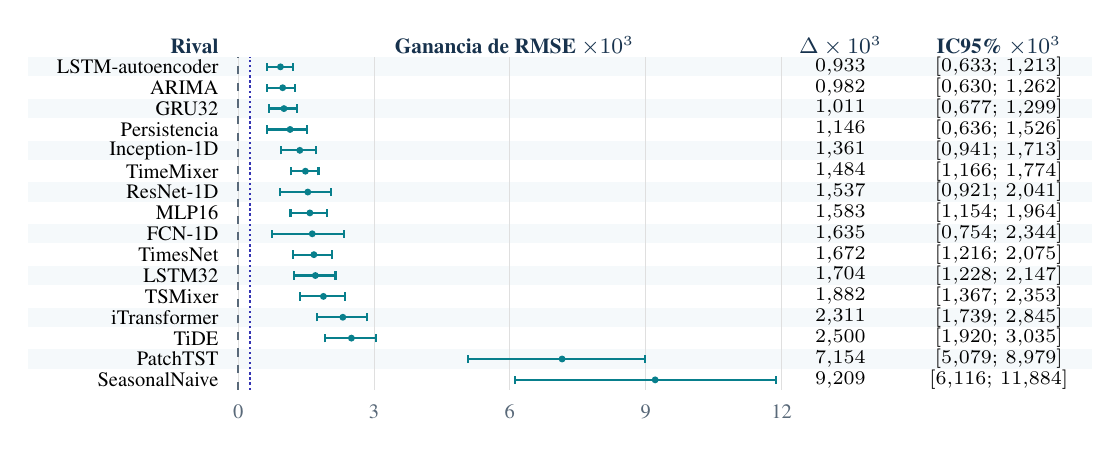
\begin{tikzpicture}[x=.575cm,y=.265cm,font=\fontsize{7.4}{8.2}\selectfont]
% Todos los puntos y límites se toman de los resultados publicados.
% La gráfica usa una única escala lineal; las cifras se multiplican por 1000.
\foreach \y in {2,4,6,8,10,12,14,16}{
  \fill[Fondo] (-4.65,\y-.46) rectangle (18.85,\y+.46);
}
\foreach \x in {0,3,6,9,12}{
  \draw[gray!25,line width=.3pt] (\x,.52) -- (\x,16.48);
  \node[anchor=north,text=Gris] at (\x,.30) {\x};
}
\draw[Gris,dashed,line width=.65pt] (0,.52) -- (0,16.48);
\draw[Azul,densely dotted,line width=.85pt] (.257728427,.52) -- (.257728427,16.48);
\node[anchor=east,text=Tinta,font=\fontsize{7.7}{8.5}\selectfont\bfseries] at (-.22,16.98) {Rival};
\node[text=Tinta,font=\fontsize{7.7}{8.5}\selectfont\bfseries] at (6.1,16.98) {Ganancia de RMSE $\times10^3$};
\node[text=Tinta,font=\fontsize{7.7}{8.5}\selectfont\bfseries] at (13.3,16.98) {$\Delta\times10^3$};
\node[text=Tinta,font=\fontsize{7.7}{8.5}\selectfont\bfseries] at (16.8,16.98) {IC95\% $\times10^3$};
\node[anchor=east] at (-.22,16) {LSTM-autoencoder};
\draw[Teal,line width=.8pt] (0.632935882,16) -- (1.213174643,16);
\draw[Teal,line width=.8pt] (0.632935882,16-.20) -- (0.632935882,16+.20);
\draw[Teal,line width=.8pt] (1.213174643,16-.20) -- (1.213174643,16+.20);
\fill[Teal] (0.933457051,16) circle[radius=1.25pt];
\node at (13.3,16) {$ 0{,}933 $};
\node at (16.8,16) {$[0{,}633;\,1{,}213]$};
\node[anchor=east] at (-.22,15) {ARIMA};
\draw[Teal,line width=.8pt] (0.629829423,15) -- (1.261897917,15);
\draw[Teal,line width=.8pt] (0.629829423,15-.20) -- (0.629829423,15+.20);
\draw[Teal,line width=.8pt] (1.261897917,15-.20) -- (1.261897917,15+.20);
\fill[Teal] (0.982192358,15) circle[radius=1.25pt];
\node at (13.3,15) {$ 0{,}982 $};
\node at (16.8,15) {$[0{,}630;\,1{,}262]$};
\node[anchor=east] at (-.22,14) {GRU32};
\draw[Teal,line width=.8pt] (0.677054034,14) -- (1.299190618,14);
\draw[Teal,line width=.8pt] (0.677054034,14-.20) -- (0.677054034,14+.20);
\draw[Teal,line width=.8pt] (1.299190618,14-.20) -- (1.299190618,14+.20);
\fill[Teal] (1.010542741,14) circle[radius=1.25pt];
\node at (13.3,14) {$ 1{,}011 $};
\node at (16.8,14) {$[0{,}677;\,1{,}299]$};
\node[anchor=east] at (-.22,13) {Persistencia};
\draw[Teal,line width=.8pt] (0.636395683,13) -- (1.526255587,13);
\draw[Teal,line width=.8pt] (0.636395683,13-.20) -- (0.636395683,13+.20);
\draw[Teal,line width=.8pt] (1.526255587,13-.20) -- (1.526255587,13+.20);
\fill[Teal] (1.146163448,13) circle[radius=1.25pt];
\node at (13.3,13) {$ 1{,}146 $};
\node at (16.8,13) {$[0{,}636;\,1{,}526]$};
\node[anchor=east] at (-.22,12) {Inception-1D};
\draw[Teal,line width=.8pt] (0.940612371,12) -- (1.713045414,12);
\draw[Teal,line width=.8pt] (0.940612371,12-.20) -- (0.940612371,12+.20);
\draw[Teal,line width=.8pt] (1.713045414,12-.20) -- (1.713045414,12+.20);
\fill[Teal] (1.360786688,12) circle[radius=1.25pt];
\node at (13.3,12) {$ 1{,}361 $};
\node at (16.8,12) {$[0{,}941;\,1{,}713]$};
\node[anchor=east] at (-.22,11) {TimeMixer};
\draw[Teal,line width=.8pt] (1.165845954,11) -- (1.773544665,11);
\draw[Teal,line width=.8pt] (1.165845954,11-.20) -- (1.165845954,11+.20);
\draw[Teal,line width=.8pt] (1.773544665,11-.20) -- (1.773544665,11+.20);
\fill[Teal] (1.483894773,11) circle[radius=1.25pt];
\node at (13.3,11) {$ 1{,}484 $};
\node at (16.8,11) {$[1{,}166;\,1{,}774]$};
\node[anchor=east] at (-.22,10) {ResNet-1D};
\draw[Teal,line width=.8pt] (0.920657426,10) -- (2.041157480,10);
\draw[Teal,line width=.8pt] (0.920657426,10-.20) -- (0.920657426,10+.20);
\draw[Teal,line width=.8pt] (2.041157480,10-.20) -- (2.041157480,10+.20);
\fill[Teal] (1.537475272,10) circle[radius=1.25pt];
\node at (13.3,10) {$ 1{,}537 $};
\node at (16.8,10) {$[0{,}921;\,2{,}041]$};
\node[anchor=east] at (-.22,9) {MLP16};
\draw[Teal,line width=.8pt] (1.153514945,9) -- (1.963664610,9);
\draw[Teal,line width=.8pt] (1.153514945,9-.20) -- (1.153514945,9+.20);
\draw[Teal,line width=.8pt] (1.963664610,9-.20) -- (1.963664610,9+.20);
\fill[Teal] (1.583441029,9) circle[radius=1.25pt];
\node at (13.3,9) {$ 1{,}583 $};
\node at (16.8,9) {$[1{,}154;\,1{,}964]$};
\node[anchor=east] at (-.22,8) {FCN-1D};
\draw[Teal,line width=.8pt] (0.753646169,8) -- (2.344102215,8);
\draw[Teal,line width=.8pt] (0.753646169,8-.20) -- (0.753646169,8+.20);
\draw[Teal,line width=.8pt] (2.344102215,8-.20) -- (2.344102215,8+.20);
\fill[Teal] (1.634895628,8) circle[radius=1.25pt];
\node at (13.3,8) {$ 1{,}635 $};
\node at (16.8,8) {$[0{,}754;\,2{,}344]$};
\node[anchor=east] at (-.22,7) {TimesNet};
\draw[Teal,line width=.8pt] (1.216162659,7) -- (2.075018985,7);
\draw[Teal,line width=.8pt] (1.216162659,7-.20) -- (1.216162659,7+.20);
\draw[Teal,line width=.8pt] (2.075018985,7-.20) -- (2.075018985,7+.20);
\fill[Teal] (1.671532105,7) circle[radius=1.25pt];
\node at (13.3,7) {$ 1{,}672 $};
\node at (16.8,7) {$[1{,}216;\,2{,}075]$};
\node[anchor=east] at (-.22,6) {LSTM32};
\draw[Teal,line width=.8pt] (1.227899168,6) -- (2.146686287,6);
\draw[Teal,line width=.8pt] (1.227899168,6-.20) -- (1.227899168,6+.20);
\draw[Teal,line width=.8pt] (2.146686287,6-.20) -- (2.146686287,6+.20);
\fill[Teal] (1.704394083,6) circle[radius=1.25pt];
\node at (13.3,6) {$ 1{,}704 $};
\node at (16.8,6) {$[1{,}228;\,2{,}147]$};
\node[anchor=east] at (-.22,5) {TSMixer};
\draw[Teal,line width=.8pt] (1.367126431,5) -- (2.352792519,5);
\draw[Teal,line width=.8pt] (1.367126431,5-.20) -- (1.367126431,5+.20);
\draw[Teal,line width=.8pt] (2.352792519,5-.20) -- (2.352792519,5+.20);
\fill[Teal] (1.882110999,5) circle[radius=1.25pt];
\node at (13.3,5) {$ 1{,}882 $};
\node at (16.8,5) {$[1{,}367;\,2{,}353]$};
\node[anchor=east] at (-.22,4) {iTransformer};
\draw[Teal,line width=.8pt] (1.738824546,4) -- (2.844863859,4);
\draw[Teal,line width=.8pt] (1.738824546,4-.20) -- (1.738824546,4+.20);
\draw[Teal,line width=.8pt] (2.844863859,4-.20) -- (2.844863859,4+.20);
\fill[Teal] (2.311247148,4) circle[radius=1.25pt];
\node at (13.3,4) {$ 2{,}311 $};
\node at (16.8,4) {$[1{,}739;\,2{,}845]$};
\node[anchor=east] at (-.22,3) {TiDE};
\draw[Teal,line width=.8pt] (1.919998936,3) -- (3.034906526,3);
\draw[Teal,line width=.8pt] (1.919998936,3-.20) -- (1.919998936,3+.20);
\draw[Teal,line width=.8pt] (3.034906526,3-.20) -- (3.034906526,3+.20);
\fill[Teal] (2.500315122,3) circle[radius=1.25pt];
\node at (13.3,3) {$ 2{,}500 $};
\node at (16.8,3) {$[1{,}920;\,3{,}035]$};
\node[anchor=east] at (-.22,2) {PatchTST};
\draw[Teal,line width=.8pt] (5.079082623,2) -- (8.978975940,2);
\draw[Teal,line width=.8pt] (5.079082623,2-.20) -- (5.079082623,2+.20);
\draw[Teal,line width=.8pt] (8.978975940,2-.20) -- (8.978975940,2+.20);
\fill[Teal] (7.153618379,2) circle[radius=1.25pt];
\node at (13.3,2) {$ 7{,}154 $};
\node at (16.8,2) {$[5{,}079;\,8{,}979]$};
\node[anchor=east] at (-.22,1) {SeasonalNaive};
\draw[Teal,line width=.8pt] (6.116205990,1) -- (11.884003400,1);
\draw[Teal,line width=.8pt] (6.116205990,1-.20) -- (6.116205990,1+.20);
\draw[Teal,line width=.8pt] (11.884003400,1-.20) -- (11.884003400,1+.20);
\fill[Teal] (9.209135448,1) circle[radius=1.25pt];
\node at (13.3,1) {$ 9{,}209 $};
\node at (16.8,1) {$[6{,}116;\,11{,}884]$};
\end{tikzpicture}\par}
\vspace{1pt}
{\fontsize{7.3}{8.4}\selectfont \textbf{Punto:} ganancia. \textbf{Barra:} intervalo de confianza. \textbf{Gris:} cero. \textbf{Azul:} margen $\delta\times10^3=0{,}258$.\par}
\idea{Los 16 intervalos marginales superan cero y $\delta$. Corresponden a la ganancia de RMSE, no al MSE de DM; no garantizan cobertura simultánea para todos los rivales.}
\fuenteURL{\HistURL/contrasts_table.csv}{Bootstrap circular pareado: bloques de 14 días, 9.999 réplicas y 608 fechas. Modelos ajustados fijos}
\end{frame}

\begin{frame}[t]{Limitaciones y siguiente comparación}
\tiempo{1:30}\compacta
\begin{columns}[T,onlytextwidth]
\column{.47\textwidth}
\begin{block}{Input-only: piloto de desarrollo}
\begin{puntos}
\item 55 fechas ya expuestas y selección posterior de la candidata.
\item Intervalos que incluyen cero y variabilidad entre cinco semillas. Los resultados históricos de DM/HLN no se transfieren a esta candidata.
\end{puntos}
\end{block}
\column{.49\textwidth}
\begin{block}{CNN-LSTM-atención: comparación histórica}
\begin{puntos}\setlength{\itemsep}{4pt}
\item Análisis retrospectivo: E2 ajusta 655 ejemplos y E3 ajusta 532, con reglas de selección distintas.
\item DM/HAC requiere dependencia débil y una varianza de largo plazo estimable. Las trayectorias entrenadas permanecen fijas.
\item Con piso común, la ventaja de RMSE frente al mejor rival baja del 24,10\% al 10,33\%.
\end{puntos}
\end{block}
\end{columns}
\smallskip
{\small Con piso común, el mejor rival es TSMixer. Los $p$ de RMSE y DM/HLN evalúan las predicciones originales.}
\smallskip\par
{\footnotesize Piloto input-only y variantes: 30 ajustes, 965 épocas, unos 76 s activos y 10 s de guardado. Registro parcial.}
\idea{Holm y HAC no corrigen la selección retrospectiva ni las diferencias de entrenamiento. La confirmación exige recetas congeladas, datos reservados y condiciones comparables.}
\fuenteURL{\DMURL}{Alcance de DM/HLN; equidad en 8.2, control del piso en 8.10 y evaluación de input-only en 8.28--8.30}
\end{frame}

\begin{frame}[t]{Conclusiones y resultados reproducibles}
\tiempo{1:00}\compacta
\begin{columns}[T,onlytextwidth]
\column{.51\textwidth}
\begin{block}{Resultados principales}
\begin{puntos}
\item \textbf{Mecanismo:} transformar la magnitud futura antes de promediar y conservar el mínimo observable.
\item \textbf{Input-only:} mejora descriptiva del 2,76\% frente a Global MSE. Sus intervalos incluyen cero.
\item \textbf{Histórico, 608 fechas:} 24,10\% menos RMSE que el mejor rival. DM-HAC14: 16/16 rechazos con Holm16 y Holm64. HLN aproximado conserva los 16.
\end{puntos}
\end{block}
\column{.45\textwidth}
\begin{block}{Consultar y reproducir}
\href{\BookURL/intro.html}{\textbf{Entregable 3 completo}}\par\medskip
\href{\BookURL/sections/08_verificacion_estadistica.html}{\textbf{Comparación numérica y estadística}}\par\medskip
\href{\DMURL}{\textbf{DM y HLN: protocolo y resultados}}\par\medskip
\href{\ResultadosURL}{\textbf{Curvas y predicciones de input-only}}\par\medskip
\href{\ModeloURL}{\textbf{Código de la arquitectura}}
\end{block}
\end{columns}
\idea{DM y HLN respaldan la ventaja histórica de CNN-LSTM-atención bajo los supuestos del análisis. Input-only conserva evidencia de desarrollo; su confirmación independiente sigue pendiente.}
\fuenteURL{\DMURL}{Análisis complementario del 25/11/2026; resultados previos en 8.5--8.7 y 8.28--8.30}
\end{frame}

\end{document}
